% \iffalse meta-comment
%
% kTheTex-bundle.dtx
% Copyright 2017 Knut Zoch <github.com/knutzk>
%
% This work may be distributed and/or modified under the conditions of
% the LaTeX Project Public License, either version 1.3 of this license
% or (at your option) any later version.  The latest version of this
% license is in http://www.latex-project.org/lppl.txt and version 1.3
% or later is part of all distributions of LaTeX version 2005/12/01 or
% later.
%
% This work has the LPPL maintenance status `maintained'.
%
% The Current Maintainer of this work is Knut Zoch.
%
% This work consists of the files kTheTex-bundle.dtx,
% kTheTex-bundle.ins, dtx/ktx-base.dtx, dtx/ktx-bibliography.dtx,
% dtx/ktx-debug.dtx, dtx/ktx-drafting.dtx, dtx/ktx-floats.dtx,
% dtx/ktx-font.dtx, dtx/ktx-headfoot.dtx, dtx/ktx-headings.dtx,
% dtx/ktx-misc-style.dtx, dtx/ktx-references.dtx,
% dtx/ktx-titlepage.dtx, dtx/ktx-toc.dtx as well as the derived files
% ktxbbltx.sty, ktxreprt.cls and ktxthss.cls.
%
% generate change history via:
% makeindex -s gglo.ist -o kTheTex-bundle.gls kTheTex-bundle.glo
%
% \fi
%
% \iffalse
%<*driver>
\ProvidesFile{process.dtx}
[2016/12/21 v0.2.0 kTheTex-bundle]
%</driver>
%<report|thesis>\NeedsTeXFormat{LaTeX2e}[2005/12/01]
%<report>\ProvidesClass{ktxreprt}
%<thesis>\ProvidesClass{ktxthss}
%<report>[2016/12/21 v0.2.0 kTheTex-bundle -- Report class]
%<thesis>[2016/12/21 v0.2.0 kTheTex-bundle -- Thesis class]
%
%<*driver>
\documentclass{ltxdoc}
\usepackage{mathpazo}
\usepackage[scaled]{helvet}
\usepackage{leading}
\leading{13pt}
\usepackage{sectsty}
\allsectionsfont{\sffamily}
\EnableCrossrefs
\CodelineIndex
\RecordChanges
\begin{document}
\DocInput{kTheTex-bundle.dtx}
\end{document}
%</driver>
% \fi
%
% \CheckSum{0}
%
% \CharacterTable
%  {Upper-case    \A\B\C\D\E\F\G\H\I\J\K\L\M\N\O\P\Q\R\S\T\U\V\W\X\Y\Z
%   Lower-case    \a\b\c\d\e\f\g\h\i\j\k\l\m\n\o\p\q\r\s\t\u\v\w\x\y\z
%   Digits        \0\1\2\3\4\5\6\7\8\9
%   Exclamation   \!     Double quote  \"     Hash (number) \#
%   Dollar        \$     Percent       \%     Ampersand     \&
%   Acute accent  \'     Left paren    \(     Right paren   \)
%   Asterisk      \*     Plus          \+     Comma         \,
%   Minus         \-     Point         \.     Solidus       \/
%   Colon         \:     Semicolon     \;     Less than     \<
%   Equals        \=     Greater than  \>     Question mark \?
%   Commercial at \@     Left bracket  \[     Backslash     \\
%   Right bracket \]     Circumflex    \^     Underscore    \_
%   Grave accent  \`     Left brace    \{     Vertical bar  \|
%   Right brace   \}     Tilde         \~}
%
%
% \changes{v0.1.0}{2016/04/18}{Initial version} %
% \GetFileInfo{process.dtx} %
% \DoNotIndex{} %
% \title{The \textsf{kTheTex-bundle}\thanks{This document
% corresponds to \textsf{kTheTex-bundle}~\fileversion,
%   dated \filedate.}}
% \author{Knut Zoch \\ \texttt{github.com/knutzk}} %
% \maketitle
%
% \iffalse
% \begin{abstract}
%   Put text here.
% \end{abstract}
% \fi
%
% \section{Introduction}
%
% This is the documentation of the |kTheTex-bundle| package
% \LaTeX. Its classes allow typesetting of reports and
% theses. Unfortunately, this documentation still lacks a concise
% description of the functionalities, but only includes descriptions
% of the implementations in the next section. Eventually, the
% documentation should look like this:
%
% \DescribeMacro{\dummyMacro}
% This macro does nothing.\index{doing nothing|usage} It is merely an
% example.  If this were a real macro, you would put a paragraph here
% describing what the macro is supposed to do, what its mandatory and
% optional arguments are, and so forth.
%
% \DescribeEnv{dummyEnv}
% This environment does nothing.  It is merely an example.
% If this were a real environment, you would put a paragraph here
% describing what the environment is supposed to do, what its
% mandatory and optional arguments are, and so forth.
%
% \StopEventually{}
%
% \section{Implementation}
% % \iffalse meta-comment
%
% ktx-base.dtx
% Copyright 2016 K. Zoch <github.com/kzoch>
%
% This work may be distributed and/or modified under the conditions of
% the LaTeX Project Public License, either version 1.3 of this license
% or (at your option) any later version.  The latest version of this
% license is in http://www.latex-project.org/lppl.txt and version 1.3
% or later is part of all distributions of LaTeX version 2005/12/01 or
% later.
%
% This work has the LPPL maintenance status `maintained'.
%
% The Current Maintainer of this work is K. Zoch.
%
% This work consists of the files kTheTex-bundle.dtx,
% kTheTex-bundle.ins, dtx/ktx-base.dtx, dtx/ktx-bibliography.dtx,
% dtx/ktx-debug.dtx, dtx/ktx-drafting.dtx, dtx/ktx-floats.dtx,
% dtx/ktx-font.dtx, dtx/ktx-headfoot.dtx, dtx/ktx-headings.dtx,
% dtx/ktx-misc-style.dtx, dtx/ktx-references.dtx, dtx/ktx-toc.dtx as
% well as the derived files ktxbbltx.sty, ktxreprt.cls and
% ktxthss.cls.
%
% \fi
%
% \iffalse
%<*driver>
\ProvidesFile{dtx/ktx-base.dtx}
[2016/04/18 v0.1.0 ktx-base]
%</driver>
%
%<*driver>
\documentclass[draft]{ltxdoc}
\EnableCrossrefs
\CodelineIndex
\RecordChanges
\changes{v0.1.0}{2016/04/18}{Initial version} %
\GetFileInfo{dtx/ktx-base.dtx} %
\DoNotIndex{} %
\title{The \textsf{kTheTex-bundle} file
\textsf{ktx-base.dtx}\thanks{This document corresponds to
\textsf{ktx-base.dtx}~\fileversion, dated \filedate.}}
\author{K. Zoch \\ \texttt{github.com/kzoch}} %
\begin{document}
\maketitle
\DocInput{dtx/ktx-base.dtx}
\end{document}
%</driver>
% \fi
%
% \CheckSum{0}
%
% \CharacterTable
%  {Upper-case    \A\B\C\D\E\F\G\H\I\J\K\L\M\N\O\P\Q\R\S\T\U\V\W\X\Y\Z
%   Lower-case    \a\b\c\d\e\f\g\h\i\j\k\l\m\n\o\p\q\r\s\t\u\v\w\x\y\z
%   Digits        \0\1\2\3\4\5\6\7\8\9
%   Exclamation   \!     Double quote  \"     Hash (number) \#
%   Dollar        \$     Percent       \%     Ampersand     \&
%   Acute accent  \'     Left paren    \(     Right paren   \)
%   Asterisk      \*     Plus          \+     Comma         \,
%   Minus         \-     Point         \.     Solidus       \/
%   Colon         \:     Semicolon     \;     Less than     \<
%   Equals        \=     Greater than  \>     Question mark \?
%   Commercial at \@     Left bracket  \[     Backslash     \\
%   Right bracket \]     Circumflex    \^     Underscore    \_
%   Grave accent  \`     Left brace    \{     Vertical bar  \|
%   Right brace   \}     Tilde         \~}
%
%
%
% Require essential packages for setting up the class options. Without
% the following packages, the basic setup will not be possible. Use a
% custom Keyval family name and prefix for internal commands (ktx is
% short and easy to remember). Provide macros for warning, info, and
% error commands to easily access them within the code.
%    \begin{macrocode}
\RequirePackage{etoolbox}[2011/01/03]
\RequirePackage{ifthen}[1999/01/07]
\RequirePackage{kvoptions}[2011/06/30]
\RequirePackage{xstring}[2012/10/24]
\SetupKeyvalOptions{%
  family=ktx,
  prefix=ktx@
}
\newcommand*{\ktx@warning}[1]{\ClassWarning{ktx}{#1}}
\newcommand*{\ktx@info}[1]{\ClassInfo{ktx}{#1}}
\newcommand*{\ktx@error}[2]{\ClassError{ktx}{#1}{#2}}
%    \end{macrocode}
% 
%
% \subsection{Declaration of Class Options}
% \label{sec:decl-class-opti}
%
% \begin{macro}{feature options}
%   Turn additional features of the class on or off.
%    \begin{macrocode}
\DeclareBoolOption[true]{biblatex}
\DeclareBoolOption[true]{hyperref}
\DeclareBoolOption[true]{microtype}
\DeclareBoolOption[true]{tocloft}
\DeclareBoolOption[true]{web}
\DeclareComplementaryOption{print}{web}
%    \end{macrocode}
% \end{macro}
%
% \begin{macro}{debug option}
%   The following option |debug| gives access to a version of the
%   class for debugging only (all unnecessary packages deactivated).
%    \begin{macrocode}
\DeclareBoolOption[false]{debug}
%    \end{macrocode}
% \end{macro}
%
% \begin{macro}{draft options}
%   Additionally, |draft| and |lightdraft| options are available.
%    \begin{macrocode}
\DeclareBoolOption[false]{draft}
\DeclareComplementaryOption{final}{draft}
\DeclareBoolOption[false]{lightdraft}
%    \end{macrocode}
% \end{macro}
%
% \begin{macro}{style options}
%   These options affect the style of the document.
%    \begin{macrocode}
\DeclareStringOption[false]{font}
\DeclareStringOption[adjust]{header}
\DeclareStringOption[sansserif]{headings}
\DeclareBoolOption[true]{pagenumberstop}
\DeclareBoolOption[false]{overlappingheadings}
%    \end{macrocode}
% \end{macro}
%
% \begin{macro}{comp options}
%   The following options are only available because there are
%   compatibility issues with the KOMA script classes. For some
%   reason, |headinclude| and |footinclude| for the geometry
%   calculation are not forwarded to the KOMA script class
%   properly. Option |ngerman| is specified to allow forwarding of the
%   language to the |prelim2e| draft package.
%    \begin{macrocode}
\DeclareBoolOption[true]{headinclude}
\DeclareBoolOption[false]{footinclude}
\DeclareBoolOption[false]{ngerman}
%    \end{macrocode}
% \end{macro}
%
%
% \subsection{Call the Base Class}
% \label{sec:call-base-class}
%
% Call the following options for the parent class:
% \begin{itemize}
% \item Put the bibliography to the table of contents.
% \item Use a font size of 11 points.
% \item Use a two-sided layout.
% \item Calculate the optimal page division factor (see KOMA script
%   documentation).
% \end{itemize}
%    \begin{macrocode}
\PassOptionsToClass{bibliography = totoc,%
                    fontsize     = 11pt,%
                    twoside      = yes,%
                    DIV          = 9,%
                    titlepage    = firstiscover,%
                    }{scrbook}
%    \end{macrocode}
%
% \noindent
% This class is based on the scrbook class from the KOMA script
% family. The class will be loaded with the following options by
% default (options in parentheses are the default values of
% scrtartcl):
%   \begin{table}[ht]
%     \centering
%     \begin{tabular}{ll}
%         bibliography = totoc   & display bibliography in TOC \\
%         BCOR         = (0mm)   & binding correction for margins \\
%         DIV          = 9       & page division factor  \\
%         fontsize     = 11pt    & set font size \\
%         footinclude  = no      & include footer in DIV calc \\
%         headinclude  = yes     & include header in DIV calc \\
%         headsepline  = (no)    & separate header+text with line \\
%         paper        = (a4)    & set paper size \\
%         titlepage    = firstiscover  & yes/no/firstiscover \\
%         twoside      = yes     & twosided/singlesided document \\
%       \end{tabular}
%       \caption{Options transferred to the base class.}
%   \label{tab:options}
% \end{table}
% 
% \noindent
% Now pass all unknown options to the base class and process all
% options (also the given default values). Then load the base class.
%    \begin{macrocode}
\DeclareDefaultOption{\PassOptionsToClass{\CurrentOption}{scrbook}}
\ProcessKeyvalOptions*
\LoadClass{scrbook}
%    \end{macrocode}
%
% \begin{macro}{hack options}
%   Hacks for passing the headinclude and footinclude options from
%   this class correctly to the base class.
%    \begin{macrocode}
\ifthenelse{\boolean{ktx@headinclude}}{%
  \KOMAoptions{headinclude=true}
}{%
  \KOMAoptions{headinclude=false}
}
\ifthenelse{\boolean{ktx@footinclude}}{%
  \KOMAoptions{footinclude=true}
}{%
  \KOMAoptions{footinclude=false}
}
%    \end{macrocode}
% \end{macro}
%

% % \iffalse meta-comment
%
% kTheTex-bundle.dtx
% Copyright 2016 Knut Zoch <knut DOT zoch AT gmail DOT com>
%
% This work may be distributed and/or modified under the conditions of the LaTeX
% Project Public License, either version 1.3 of this license or (at your option)
% any later version.  The latest version of this license is in
% http://www.latex-project.org/lppl.txt and version 1.3 or later is part of all
% distributions of LaTeX version 2005/12/01 or later.
%
% This work has the LPPL maintenance status `maintained'.
%
% The Current Maintainer of this work is Knut Zoch.
%
% This work consists of the files kTheTex-bundle.dtx, kTheTex-bundle.ins,
% dtx/ktx-base.dtx, dtx/ktx-bibliography.dtx, dtx/ktx-debug.dtx,
% dtx/ktx-drafting.dtx, dtx/ktx-floats.dtx, dtx/ktx-font.dtx,
% dtx/ktx-headfoot.dtx, dtx/ktx-headings.dtx, dtx/ktx-misc-style.dtx,
% dtx/ktx-references.dtx, dtx/ktx-toc.dtx and the derived file ktxreprt.sty.
% \fi
%
% \iffalse
%<*driver>
\ProvidesFile{dtx/ktx-debug.dtx}
[2016/04/01 v0.1 ktx-debug]
%</driver>
%
%<*driver>
\documentclass[draft]{ltxdoc}
\EnableCrossrefs
\CodelineIndex
\RecordChanges
\begin{document}
\DocInput{dtx/ktx-debug.dtx}
\end{document}
%</driver>
% \fi
%
% \CheckSum{0}
%
% \CharacterTable
%  {Upper-case    \A\B\C\D\E\F\G\H\I\J\K\L\M\N\O\P\Q\R\S\T\U\V\W\X\Y\Z
%   Lower-case    \a\b\c\d\e\f\g\h\i\j\k\l\m\n\o\p\q\r\s\t\u\v\w\x\y\z
%   Digits        \0\1\2\3\4\5\6\7\8\9
%   Exclamation   \!     Double quote  \"     Hash (number) \#
%   Dollar        \$     Percent       \%     Ampersand     \&
%   Acute accent  \'     Left paren    \(     Right paren   \)
%   Asterisk      \*     Plus          \+     Comma         \,
%   Minus         \-     Point         \.     Solidus       \/
%   Colon         \:     Semicolon     \;     Less than     \<
%   Equals        \=     Greater than  \>     Question mark \?
%   Commercial at \@     Left bracket  \[     Backslash     \\
%   Right bracket \]     Circumflex    \^     Underscore    \_
%   Grave accent  \`     Left brace    \{     Vertical bar  \|
%   Right brace   \}     Tilde         \~}
%
%
% \changes{v1.0}{2016/03/25}{Initial version} %
% \GetFileInfo{dtx/ktx-debug.dtx} %
% \DoNotIndex{} %
%
% \title{The \textsf{kTheTex-bundle} file
% \textsf{ktx-debug.dtx}\thanks{This document corresponds to
% \textsf{ktx-debug.dtx}~\fileversion, dated \filedate.}}
% \author{Knut Zoch \\ \texttt{knut.zoch NOSPAM gmail.com}} %
% \maketitle
%
%
% \subsection{Debugging}
% \label{sec:debugging}
%
% \begin{macro}{debug}
%   If option |debug| is set, then the code will stop after the
%   following lines. DEBUG: this should probably contain more (does it
%   crash?).
%    \begin{macrocode}
\ifthenelse{\boolean{ktx@debug}}{%
  \usepackage{amsmath,graphicx,float,biblatex}
  \let\cref\relax
  \let\href\relax
  \let\setstretch\relax
  \let\toprule\relax
  \let\midrule\relax
  \let\bottomrule\relax
  \let\textscl\textsc
  \let\textsca\textsc
  \newcommand*{\subcaptionbox}[2][]{}
  \endinput
}{%
  \relax
}
%    \end{macrocode}
% \end{macro}
%

% %
% \subsection{Fonts}
% \label{sec:fonts}
%
% In this section, a couple of fonts are proposed and their settings optimised for usage with this class. The fonts can be chosen with the option |fonts|. Currently, three types are available: MinionPro (proprietary), Kepler fonts, mathpazo.
%
%    \begin{macrocode}
\IfEqCase*{\ktxreprt@font}{%
%    \end{macrocode}
%
% \begin{macro}{font=minion}
%   Choose MinionPro as the main font and MyriadPro as a supplementing
%   sans-serif font for the main text. Those fonts are only available as
%   proprietary fonts, so make sure your system provides them first!
%
%   The given options include old-style numerals, custom MinionPro integral
%   symbols, swashed italics capitals and Greek italics (also for the Greek
%   capital letters).
%    \begin{macrocode}
  {minion}{%
    \RequirePackage{MnSymbol}%
    \RequirePackage[mathlf,%
                    textosf,%
                    minionint,%
                    swash,%
                    italicgreek,%
                    ]{MinionPro}%
    \RequirePackage[lf,scale=0.92,sansmath]{MyriadPro}}%
%    \end{macrocode}
% \end{macro}
%
% \begin{macro}{font=kpfonts}
%   Load the package |kpfonts| for the main font and |berasans| for the
%   sans-serif font. Given options include slanted Greek letters, old-style
%   numerals and the partial derivative symbol non-slanted.
%    \begin{macrocode}
  {kpfonts}{%
    \RequirePackage[slantedGreeks,oldstylenums,partialup]{kpfonts}%
    \RequirePackage[scaled=0.86]{berasans}}%
%    \end{macrocode}
% \end{macro}
%
% \begin{macro}{font=mathpazo}
%   Load the package |mathpazo| for the main font and |helvet| (Helvetica) for
%   the sans-serif font. Use a scaled version for the latter one.
%    \begin{macrocode}
  {mathpazo}{%
    \RequirePackage{mathpazo}%
    \RequirePackage[scaled]{helvet}}%
%    \end{macrocode}
% \end{macro}
%
% \begin{macro}{font=false}
%   Do nothing here. This leaves the choice of the font to the user -- otherwise
%   the standard font Computer Modern will be used.
%    \begin{macrocode}
  {false}{}%
%    \end{macrocode}
% \end{macro}
%
% \noindent
% Issue an error when the given font type is unknown.
%    \begin{macrocode}
}[\ktxreprt@error{Unknown font: "\ktxreprt@font"}{%
  The given font is unknown. ktxreprt class supports the fonts kpfonts,
  mathpazo, minion and CM. If you want to use your own font
  declarations, use option "font=false".}]
%    \end{macrocode}
%

% %
% \subsection{Draft Settings}
% \label{sec:draft-settings}
%
% This section introduces a couple of packages and settings that will be
% activated only for the options |draft| or |lightdraft| (a draft version
% without the distracting rulers at the top and bottom of the pages).
%
% First define a warning that will be issued for option |lightdraft| since this
% is a class-specific feature.
%
%    \begin{macrocode}
\newcommand*{\issuelightdraftwarning}{\ktx@warning{%
    Option "lightdraft" is set. To get full draft features,\MessageBreak
    set option "draft" (and deactivate "lightdraft"). If \MessageBreak
    this is meant to be a final version, deactivate the \MessageBreak
    lightdraft and draft option or set the option "final".\MessageBreak}
}
%    \end{macrocode}
%
% \begin{macro}{lightdraft}
%   If the option |lightdraft| is set, also switch the boolean |draft| to
%   |true|. The only real difference is that the underlying KOMA script class
%   won't notice that draft features are used. Otherwise, the rulers would be
%   switched on.
%    \begin{macrocode}
\ifthenelse{\boolean{ktx@lightdraft}}{%
  \setboolean{ktx@draft}{true}
}{}
%    \end{macrocode}
% \end{macro}
%
% \begin{macro}{draft}
%   Now the custom features for the draft option are set. This includes a draft
%   watermark with the package |draftwatermark| that will be set in the
%   background of every page. The package |prelim2e| sets a draft notice at the
%   very bottom of every page.
%    \begin{macrocode}
\ifthenelse{\boolean{ktx@draft}}{%
  \RequirePackage{draftwatermark}%
  \SetWatermarkLightness{0.9}%
  \SetWatermarkScale{0.7}%
  \SetWatermarkText{Preliminary}%
  \ifthenelse{\boolean{ktx@ngerman}}{%
    \PassOptionsToPackage{german}{prelim2e}%
  }{}%
  \RequirePackage[scrtime]{prelim2e}%
%    \end{macrocode}
% Now crosscheck whether the lightdraft option is set and forward that
% information to KOMA script. KOMA will only use draft settings if |draft| is
% set, NOT for |lightdraft|. For the traditional |draft| option, the package
% |showframe| will also be loaded to display a frame around the text areas.
%    \begin{macrocode}
  \ifthenelse{\boolean{ktx@lightdraft}}{%
    \issuelightdraftwarning
    \KOMAoptions{draft=false}
  }{
    \RequirePackage{showframe}%
    \KOMAoptions{draft=true}%
  }
%    \end{macrocode}
% If the boolean |draft| is set to false, also make sure that KOMA script will
% get this message.
%    \begin{macrocode}
}{%
  \KOMAoptions{draft=false}
}
%    \end{macrocode}
% \end{macro}
%

% %
% \subsection{Miscellaneous Page Style}
% \label{sec:misc-page-style}
%
% \begin{macro}{microtype}
%   Optimise text spread with microtype package. First make a check whether the
%   |microtype| option has been set.
%    \begin{macrocode}
\ifthenelse{\boolean{ktx@microtype}}{%
%    \end{macrocode}
% Now load package |microtype|. Options include: use language information from
% the babel package to determine kerning etc. Set stretch and shrink to a value
% of 10 (20 is default). And always use final=true, i.e. ignore draft options
% from the class in order to \emph{always} run |microtype|. To really turn it
% off, use the option |microtype=false|.
%    \begin{macrocode}
  \RequirePackage[babel   = true,%
                  stretch = 10,%
                  shrink  = 10,%
                  final   = true,%
                  ]{microtype}
%    \end{macrocode}
% Issue a warning if package |microtype| is not loaded.
%    \begin{macrocode}
 }{%
   \ktx@warning{Microtype package not loaded.}
}
%    \end{macrocode}
% \end{macro}
%
% \begin{macro}{letterspacing}
%   Now adjust the letter spacing for the small-caps font (in the standard
%   settings, the spacing is way too small). For that, use the |microtype|
%   package. First, check if |microtype| was loaded or not. If this is not the
%   case, load the package |letterspacing| which is part of the |microtype|
%   package. Maybe the latter one was turned off deliberately, so we only want
%   the letter spacing features here. 
%    \begin{macrocode}
\@ifpackageloaded{microtype}{
  \relax
}{%
  \RequirePackage{letterspace}}
%    \end{macrocode}
% Now first provide commands for fully-capitalised and only-small-caps fonts. By
% default, those commands work fine, but always issue a warning because the
% spacing is not adjusted.
%    \begin{macrocode}
\newrobustcmd{\ktx@allcaps}[1]{%
  \ktx@warning{Spacing of small caps not adjusted! Using
    default\MessageBreak spacing now.}\textsc{\MakeUppercase{#1}}}
\newrobustcmd{\ktx@lowcaps}[1]{%
  \ktx@warning{Spacing of small caps not adjusted! Using
    default\MessageBreak spacing now.}\textsc{\MakeLowercase{#1}}}
%    \end{macrocode}
% Check if either |letterspacing| or |microtype| were loaded before applying the
% spacing corrections.
%    \begin{macrocode}
\ifboolexpr{ test {\@ifpackageloaded{letterspace}} or
             test {\@ifpackageloaded{microtype}} }{%
  \ktx@info{Using letterspacing options of microtype package.}
  \renewrobustcmd{\ktx@allcaps}[1]{%
                  \textls[150]{\MakeUppercase{#1}}}
  \renewrobustcmd{\ktx@lowcaps}[1]{%
                  \textls[50]{\textsc{\MakeLowercase{#1}}}}
%    \end{macrocode}
% Also apply the spacing corrections for the standard |\textsc| command.
%    \begin{macrocode}
  \let\ktx@textsc@old\textsc
  \renewcommand*{\textsc}[1]{\textls[50]{\ktx@textsc@old{#1}}}
%    \end{macrocode}
% If none of the packages was loaded, do nothing (warnings will be printed when
% all-caps or low-caps are used).
%    \begin{macrocode}
}{%
  \relax
}
%    \end{macrocode}
% Finally, provide global commands for the defined fonts: |\textsca| and
% |\textscl|.
%    \begin{macrocode}
\let\textsca\ktx@allcaps
\let\textscl\ktx@lowcaps
%    \end{macrocode}
% \end{macro}
%
%
% \subsection{Trash Section}
% \label{sec:trash-section}
%
% \begin{macro}{alles}
%   DEBUG BESCHREIBUNG FEHLT
%    \begin{macrocode}
\linespread{1.12}
\KOMAoptions{DIV=last}
%    \end{macrocode}
% \end{macro}
% 
% \begin{macro}{alles}
%   Declare essential text formatting commands (robust, no dependencies).
%    \begin{macrocode}
\newcommand*{\ktx@textsw}[1]{\textit{#1}}
\newcommand*{\ktx@swshape}{\itshape}
\ifdefstring{\ktx@font}{minion}{%
  \renewcommand*{\ktx@textsw}[1]{\textsw{#1}}
  \renewcommand*{\ktx@swshape}{\swshape}
}{}
%    \end{macrocode}
% \end{macro}
%
% \begin{macro}{alles}
%    \begin{macrocode}
\RequirePackage[utf8]{inputenc}         % encoding of document is UTF8
\RequirePackage{babel}                  % language support (hyphenation etc.)
\RequirePackage{amsmath}                % math package
\RequirePackage[autostyle=true]{csquotes} % sync quoting style with language
\RequirePackage{enumitem}               % control layout of lists
\RequirePackage[T1]{fontenc}            % fontenc T1 (includes Umlaute)
\RequirePackage{graphicx}               % support for graphics inclusion
\RequirePackage{xcolor}                 % support for custom colours
\RequirePackage{xspace}                 % custom commands do not eat spaces
%    \end{macrocode}
% \end{macro}
%
% \begin{macro}{alles}
%    \begin{macrocode}
%<*report>
\numberwithin{equation}{section}
\numberwithin{table}{section}
\numberwithin{figure}{section}
%</report>
%<*thesis>
\numberwithin{equation}{chapter}
\numberwithin{table}{chapter}
\numberwithin{figure}{chapter}
%</thesis>
% \definecolor{Maroon}{cmyk}{0, 0.87, 0.68, 0.32}
% \definecolor{RoyalBlue}{cmyk}{1, 0.5, 0, 0}
% \definecolor{Black}{cmyk}{0, 0, 0, 0}
% \definecolor{webgreen}{cmyk}{1, 0, 1, 0.5}
% \definecolor{webbrown}{cmyk}{0, 1, 1, 0.4}
% Name still preliminary
\definecolor{Venetian}{cmyk}{0, 0.95, 0.85, 0.30}
\definecolor{Lime}{cmyk}{0.85, 0, 0.75, 0.25}
\definecolor{Dodger}{cmyk}{1, 0.40, 0, 0.10}
\graphicspath{{./figures/}}             % ==> look for figures in folder
\setlist{itemsep=-1ex}                 % ==> smaller spacing between items
\setlist[enumerate]{itemsep=0.1\baselineskip}
\setlist{leftmargin=1.5em}
\setlength{\parskip}{0pt}% plus 0.3\baselineskip}
\setlist{nosep}
%% This might be interesting for an option to change to articles
%% (no chapters)
%% \renewcommand*\thesection{\arabic{section}}
%    \end{macrocode}
% \end{macro}
%
% \begin{macro}{alles}
%   Alter some LaTeX defaults for better treatment of figures: See p.105 of "TeX Unbound" for suggested values. See pp. 199-200 of Lamport's "LaTeX" book for details. General parameters, for ALL pages:
%    \begin{macrocode}
\renewcommand{\topfraction}{0.9}	% max fraction of floats at top
\renewcommand{\bottomfraction}{0.8}	% max fraction of floats at bottom
%    \end{macrocode}
% Parameters for TEXT pages (not float pages):
%    \begin{macrocode}
\setcounter{topnumber}{2}
\setcounter{bottomnumber}{2}
\setcounter{totalnumber}{4}             % 2 may work better
\setcounter{dbltopnumber}{2}            % for 2-column pages
\renewcommand{\dbltopfraction}{0.9}	% fit big float above 2-col. text
\renewcommand{\textfraction}{0.07}	% allow minimal text w. figs
%    \end{macrocode}
% Parameters for FLOAT pages (not text pages):
%    \begin{macrocode}
\renewcommand{\floatpagefraction}{0.7}	% require fuller float pages
%    \end{macrocode}
% N.B.: floatpagefraction MUST be less than topfraction !!
%    \begin{macrocode}
\renewcommand{\dblfloatpagefraction}{0.7}	% require fuller float pages
%    \end{macrocode}
% \end{macro}
% 

% % \iffalse meta-comment
%
% ktx-headings.dtx
% Copyright 2016 Knut Zoch <knut DOT zoch AT gmail DOT com>
%
% This work may be distributed and/or modified under the conditions of
% the LaTeX Project Public License, either version 1.3 of this license
% or (at your option) any later version.  The latest version of this
% license is in http://www.latex-project.org/lppl.txt and version 1.3
% or later is part of all distributions of LaTeX version 2005/12/01 or
% later.
%
% This work has the LPPL maintenance status `maintained'.
%
% The Current Maintainer of this work is Knut Zoch.
%
% This work consists of the files kTheTex-bundle.dtx,
% kTheTex-bundle.ins, dtx/ktx-base.dtx, dtx/ktx-bibliography.dtx,
% dtx/ktx-debug.dtx, dtx/ktx-drafting.dtx, dtx/ktx-floats.dtx,
% dtx/ktx-font.dtx, dtx/ktx-headfoot.dtx, dtx/ktx-headings.dtx,
% dtx/ktx-misc-style.dtx, dtx/ktx-references.dtx, dtx/ktx-toc.dtx as
% well as the derived files ktxbbltx.sty, ktxreprt.cls and
% ktxthss.cls.
%
% \fi
%
% \iffalse
%<*driver>
\ProvidesFile{dtx/ktx-headings.dtx}
[2016/04/18 v0.1.0 ktx-headings]
%</driver>
%
%<*driver>
\documentclass[draft]{ltxdoc}
\EnableCrossrefs
\CodelineIndex
\RecordChanges
\changes{v0.1.0}{2016/04/18}{Initial version} %
\GetFileInfo{dtx/ktx-headings.dtx} %
\DoNotIndex{} %
\title{The \textsf{kTheTex-bundle} file
  \textsf{ktx-headings.dtx}\thanks{This document corresponds to
    \textsf{ktx-headings.dtx}~\fileversion, dated \filedate.}}
\author{Knut Zoch \\ \texttt{knut.zoch NOSPAM gmail.com}} %
\begin{document}
\maketitle
\DocInput{dtx/ktx-headings.dtx}
\end{document}
%</driver>
% \fi
%
% \CheckSum{0}
%
% \CharacterTable
%  {Upper-case    \A\B\C\D\E\F\G\H\I\J\K\L\M\N\O\P\Q\R\S\T\U\V\W\X\Y\Z
%   Lower-case    \a\b\c\d\e\f\g\h\i\j\k\l\m\n\o\p\q\r\s\t\u\v\w\x\y\z
%   Digits        \0\1\2\3\4\5\6\7\8\9
%   Exclamation   \!     Double quote  \"     Hash (number) \#
%   Dollar        \$     Percent       \%     Ampersand     \&
%   Acute accent  \'     Left paren    \(     Right paren   \)
%   Asterisk      \*     Plus          \+     Comma         \,
%   Minus         \-     Point         \.     Solidus       \/
%   Colon         \:     Semicolon     \;     Less than     \<
%   Equals        \=     Greater than  \>     Question mark \?
%   Commercial at \@     Left bracket  \[     Backslash     \\
%   Right bracket \]     Circumflex    \^     Underscore    \_
%   Grave accent  \`     Left brace    \{     Vertical bar  \|
%   Right brace   \}     Tilde         \~}
%
%
%
% \subsection{Headings}
% \label{sec:headings}
%
% In this section, the headings for the documents are fixed. In a first check,
% the option |overlappingheadings| is checked that puts the number of the
% headings into the left margins of the pages. Then the headings are adjusted
% according to the givn options |headings|.
%
% \begin{macro}{overlappingheadings}
%   Check if headings are set to be overlapping or not
%    \begin{macrocode}
\let\ktx@sectionformat\sectionformat
\let\ktx@subsectionformat\subsectionformat
\let\ktx@subsubsectionformat\subsubsectionformat
%<*options>
\ifthenelse{\boolean{ktx@overlappingheadings}}{
  \renewcommand*{\ktx@sectionformat}{%
    \llap{\thesection\autodot\enskip}}
  \renewcommand*{\ktx@subsectionformat}{%
    \llap{\thesubsection\autodot\enskip}}
  \renewcommand*{\ktx@subsubsectionformat}{%
    \llap{\thesubsubsection\autodot\enskip}}
}{}
%</options>
%    \end{macrocode}
% \end{macro}
%
%
% \begin{macro}{headings}
%
% Now the adjustment to the specified headings style starts. Style |bringhurst|
% follows the style of Bringhurst's headings in his book about
% typography. |bringhurstlarge| is a scaled version of that. Other possible
% options are |italics| and |sansserif|, with the latter one being the
% standard. If no adjustments to the headings are supposed to be made by the
% class, use option |headings=false|.
%
% Each option by itself checks if |header=adjust| is set and then sets the
% correct header type according to the style of the headings. See in that
% section for more documentation.
%
% DEBUG: Not completely sure yet, whether the possibility to generate it with
% options is a good idea or not.
%
%    \begin{macrocode}
%<*options>
\IfEqCase*{\ktx@headings}{%
  {bringhurst}{%
    \renewcommand*{\sectionformat}{\ktx@sectionformat}%
    \renewcommand*{\subsectionformat}{\ktx@subsectionformat}%
    \renewcommand*{\subsubsectionformat}{\ktx@subsubsectionformat}%
    \addtokomafont{sectioning}{\normalsize\mdseries\rmfamily}%
    \setkomafont{section}{\ktx@lowcaps}%
    \setkomafont{subsection}{\ktx@swshape}%
    \setkomafont{subsubsection}{\ktx@swshape}%
    \setkomafont{paragraph}{\textsc}%
    \addtokomafont{pagehead}{\small}%
    \RedeclareSectionCommand[%
       beforeskip=-1\baselineskip plus 0.3\baselineskip,%
       afterskip=1\baselineskip,%
       ]{section}
    \RedeclareSectionCommand[%
       beforeskip=-1\baselineskip,%
       afterskip=1\baselineskip plus 0.3\baselineskip,%
       ]{subsection}
    \RedeclareSectionCommand[%
       beforeskip=-1\baselineskip,%
       afterskip=1\baselineskip,%
       ]{subsubsection}
    \RedeclareSectionCommand[%
       beforeskip=-1\baselineskip,%
       ]{paragraph}
    \ifdefstring{\ktx@header}{adjust}{%
      \renewcommand*{\ktx@header}{bringhurst}
    }{}%
  }%
  {bringhurstlarge}{%
    \renewcommand*{\sectionformat}{\ktx@sectionformat}%
    \renewcommand*{\subsectionformat}{\ktx@subsectionformat}%
    \renewcommand*{\subsubsectionformat}{\ktx@subsubsectionformat}%
    \addtokomafont{disposition}{\mdseries\rmfamily}%
    \addtokomafont{section}{\ktx@lowcaps}%
    \addtokomafont{subsection}{\ktx@swshape}%
    \addtokomafont{subsubsection}{\ktx@swshape}%
    \addtokomafont{paragraph}{\normalsize\textsc}%
    \RedeclareSectionCommand[afterskip=-0.5em]{paragraph}
    \addtokomafont{pagehead}{\small}%
    \ifdefstring{\ktx@header}{adjust}{%
      \renewcommand*{\ktx@header}{bringhurst}
    }{}%
  }%
  {italics}{%
    \renewcommand*{\sectionformat}{\ktx@sectionformat}%
    \renewcommand*{\subsectionformat}{\ktx@subsectionformat}%
    \renewcommand*{\subsubsectionformat}{\ktx@subsubsectionformat}%
    \addtokomafont{disposition}{\mdseries\rmfamily\ktx@swshape}%
    \RedeclareSectionCommand[afterskip=-0.5em]{paragraph}
    \ifdefstring{\ktx@header}{adjust}{%
      \renewcommand*{\ktx@header}{italics}
    }{}
  }%
  {sansserif}{%
%</options>
    \addtokomafont{disposition}{\bfseries\sffamily}
    \addtokomafont{title}{\color{black}}
    \renewcommand*{\sectionformat}{\ktx@sectionformat}%
    \renewcommand*{\subsectionformat}{\ktx@subsectionformat}%
    \renewcommand*{\subsubsectionformat}{\ktx@subsubsectionformat}%
    \setkomafont{paragraph}{\normalsize\mdseries\rmfamily\textscl}%
    \RedeclareSectionCommand[afterskip=-0.5em]{paragraph}
%<*options>
    \ifdefstring{\ktx@header}{adjust}{%
      \renewcommand*{\ktx@header}{sansserif}
    }{}
  }%
  {default}{}%
}[\ktx@error{unknown heading style heading=\ktx@headings}{}]
%</options>
%    \end{macrocode}
% \end{macro}
%

% % \iffalse meta-comment
%
% ktx-headfoot.dtx
% Copyright 2016 Knut Zoch <github.com/knutzk>
%
% This work may be distributed and/or modified under the conditions of
% the LaTeX Project Public License, either version 1.3 of this license
% or (at your option) any later version.  The latest version of this
% license is in http://www.latex-project.org/lppl.txt and version 1.3
% or later is part of all distributions of LaTeX version 2005/12/01 or
% later.
%
% This work has the LPPL maintenance status `maintained'.
%
% The Current Maintainer of this work is Knut Zoch.
%
% This work consists of the files kTheTex-bundle.dtx,
% kTheTex-bundle.ins, dtx/ktx-base.dtx, dtx/ktx-bibliography.dtx,
% dtx/ktx-debug.dtx, dtx/ktx-drafting.dtx, dtx/ktx-floats.dtx,
% dtx/ktx-font.dtx, dtx/ktx-headfoot.dtx, dtx/ktx-headings.dtx,
% dtx/ktx-misc-style.dtx, dtx/ktx-references.dtx,
% dtx/ktx-titlepage.dtx, dtx/ktx-toc.dtx as well as the derived files
% ktxbbltx.sty, ktxreprt.cls and ktxthss.cls.
%
% \fi
%
% \iffalse
%<*driver>
\ProvidesFile{dtx/ktx-headfoot.dtx}
[2016/12/21 v0.2.0 ktx-headfoot]
%</driver>
%
%<*driver>
\documentclass[draft]{ltxdoc}
\EnableCrossrefs
\CodelineIndex
\RecordChanges
\changes{v0.1.0}{2016/04/18}{Initial version} %
\GetFileInfo{dtx/ktx-headfoot.dtx} %
\DoNotIndex{} %
\title{The \textsf{kTheTex-bundle} file
  \textsf{ktx-headfoot.dtx}\thanks{This document corresponds to
    \textsf{ktx-headfoot.dtx}~\fileversion, dated \filedate.}}
\author{Knut Zoch \\ \texttt{github.com/knutzk}} %
\begin{document}
\maketitle
\DocInput{dtx/ktx-headfoot.dtx}
\end{document}
%</driver>
% \fi
%
% \CheckSum{0}
%
% \CharacterTable
%  {Upper-case    \A\B\C\D\E\F\G\H\I\J\K\L\M\N\O\P\Q\R\S\T\U\V\W\X\Y\Z
%   Lower-case    \a\b\c\d\e\f\g\h\i\j\k\l\m\n\o\p\q\r\s\t\u\v\w\x\y\z
%   Digits        \0\1\2\3\4\5\6\7\8\9
%   Exclamation   \!     Double quote  \"     Hash (number) \#
%   Dollar        \$     Percent       \%     Ampersand     \&
%   Acute accent  \'     Left paren    \(     Right paren   \)
%   Asterisk      \*     Plus          \+     Comma         \,
%   Minus         \-     Point         \.     Solidus       \/
%   Colon         \:     Semicolon     \;     Less than     \<
%   Equals        \=     Greater than  \>     Question mark \?
%   Commercial at \@     Left bracket  \[     Backslash     \\
%   Right bracket \]     Circumflex    \^     Underscore    \_
%   Grave accent  \`     Left brace    \{     Vertical bar  \|
%   Right brace   \}     Tilde         \~}
%
%
%
% \subsection{Headers \& Footers}
% \label{sec:headers--footers}
%
% Load the KOMA script package which is responsible for the
% header/footer design of a document: |scrlayer-scrpage|. Set the
% style of the pages to running heads by using |scrheadings| and mark
% the chapter and section titles to be put in the headers of the
% pages.
%
%    \begin{macrocode}
\RequirePackage{scrlayer-scrpage}
\pagestyle{scrheadings}
\automark[section]{chapter}
%    \end{macrocode}
%
%
% \subsubsection{Where to Put the Page Numbers}
% \label{sec:where-put-page}
%
% At first, the option |pagenumberstop| is checked. When the option is
% set to true, the page numbers will be put in the outer margin next
% to the running heads. Otherwise, the page numbers will appear in the
% outer footer (standard).
%
% First define the custom commands to put the page numbers in the
% margin. Then check whether the option has been set, put the page
% numbers to the margin and clear the footer. Finally, renew the
% commands for the left and right heads.
%    \begin{macrocode}
\let\ktx@thepage@l\empty
\let\ktx@thepage@r\empty
\ifthenelse{\boolean{ktx@pagenumberstop}}{%
  \renewcommand*{\ktx@thepage@l}{\llap{\thepage\kern1.5em}}
  \renewcommand*{\ktx@thepage@r}{\rlap{\kern1.5em\thepage}}
  \ofoot[]{}
  \cfoot[]{}
}{}
\lehead[\ktx@thepage@l]{\ktx@thepage@l\headmark}
\rohead[\ktx@thepage@r]{\headmark\ktx@thepage@r}
\chead[]{}
%    \end{macrocode}
%
%
% \subsubsection{Fix the Header Style}
% \label{sec:fix-header-style}
%
% In this part of the code, the headers and footers are
% fixed. Depending on the settings of the previous section, the
% headers may be adjusted to the headings style (then the option was
% initially set to |header=adjust| and was changed while the headings
% were fixed. Otherwise, the style can be set to the following
% options:
%
% \begin{itemize}
% \item |bringhurst|: This style follows the style of the headings
%   that are used by Bringhurst. If the option |pagenumberstop| is
%   set, the page numbers will be within the outer margin of the
%   pages.
% \item |italics|: Set the running heads to \textit{Italics}.
% \item |swash|: This style sets the running heads to the \emph{swash}
%   letters (depending on the chosen font, this might be the same as
%   the italics option).
% \item |sansserif|: And the sans-serif option, again including the
%   page numbers in the outer margin if |pagenumberstop| is set. The
%   header is also separated from the main text by a thin line.
% \item |default|: Do not adjust anything (whatever was set before is
% used).
% \item DEBUG: Here should come an error message because the
%   adjustment should have been set in the previous section already.
% \end{itemize}
%
% If the given option is unknown, return an error.
%
%    \begin{macrocode}
%<*options>
\IfEqCase*{\ktx@header}{%
  {bringhurst}{%
    \lehead{\small\ktx@thepage@l\upshape%
            \ktx@lowcaps{\headmark}}%
    \rohead{\small\ktx@textsw{\headmark}\ktx@thepage@r}}%
  {italics}{%
    \addtokomafont{pagehead}{\small\itshape}}%
  {swash}{%
    \addtokomafont{pagehead}{\small\ktx@swshape}}%
  {sansserif}{%
%</options>
\KOMAoptions{headsepline}
\setkomafont{pagehead}{\sffamily\upshape\footnotesize}
\lehead[\ktx@thepage@l]{\ktx@thepage@l\ktx@allcaps{\headmark}}
\rohead[\ktx@thepage@r]{\ktx@allcaps{\headmark}\ktx@thepage@r}
%<*options>
  }%
  {default}{}%
  {adjust}{}%
}[\ktx@error{Unknown option header=\ktx@header}{}]
%</options>
%    \end{macrocode}
%

% % \iffalse meta-comment
%
% kTheTex-bundle.dtx
% Copyright 2016 Knut Zoch <knut DOT zoch AT gmail DOT com>
%
% This work may be distributed and/or modified under the conditions of the LaTeX
% Project Public License, either version 1.3 of this license or (at your option)
% any later version.  The latest version of this license is in
% http://www.latex-project.org/lppl.txt and version 1.3 or later is part of all
% distributions of LaTeX version 2005/12/01 or later.
%
% This work has the LPPL maintenance status `maintained'.
%
% The Current Maintainer of this work is Knut Zoch.
%
% This work consists of the files kTheTex-bundle.dtx, kTheTex-bundle.ins,
% dtx/ktx-base.dtx, dtx/ktx-bibliography.dtx, dtx/ktx-debug.dtx,
% dtx/ktx-drafting.dtx, dtx/ktx-floats.dtx, dtx/ktx-font.dtx,
% dtx/ktx-headfoot.dtx, dtx/ktx-headings.dtx, dtx/ktx-misc-style.dtx,
% dtx/ktx-references.dtx, dtx/ktx-toc.dtx and the derived file ktxreprt.sty.
% \fi
%
% \iffalse
%<*driver>
\ProvidesFile{dtx/ktx-floats.dtx}
[2016/04/01 v0.1 ktx-floats]
%</driver>
%
%<*driver>
\documentclass[draft]{ltxdoc}
\EnableCrossrefs
\CodelineIndex
\RecordChanges
\changes{v1.0}{2016/03/25}{Initial version} %
\GetFileInfo{dtx/ktx-floats.dtx} %
\DoNotIndex{} %
\title{The \textsf{kTheTex-bundle} file
  \textsf{ktx-floats.dtx}\thanks{This document corresponds to
    \textsf{ktx-floats.dtx}~\fileversion, dated \filedate.}}
\author{Knut Zoch \\ \texttt{knut.zoch NOSPAM gmail.com}} %
\begin{document}
\maketitle
\DocInput{dtx/ktx-floats.dtx}
\end{document}
%</driver>
% \fi
%
% \CheckSum{0}
%
% \CharacterTable
%  {Upper-case    \A\B\C\D\E\F\G\H\I\J\K\L\M\N\O\P\Q\R\S\T\U\V\W\X\Y\Z
%   Lower-case    \a\b\c\d\e\f\g\h\i\j\k\l\m\n\o\p\q\r\s\t\u\v\w\x\y\z
%   Digits        \0\1\2\3\4\5\6\7\8\9
%   Exclamation   \!     Double quote  \"     Hash (number) \#
%   Dollar        \$     Percent       \%     Ampersand     \&
%   Acute accent  \'     Left paren    \(     Right paren   \)
%   Asterisk      \*     Plus          \+     Comma         \,
%   Minus         \-     Point         \.     Solidus       \/
%   Colon         \:     Semicolon     \;     Less than     \<
%   Equals        \=     Greater than  \>     Question mark \?
%   Commercial at \@     Left bracket  \[     Backslash     \\
%   Right bracket \]     Circumflex    \^     Underscore    \_
%   Grave accent  \`     Left brace    \{     Vertical bar  \|
%   Right brace   \}     Tilde         \~}
%
%
%
% \subsection{Floats}
% \label{sec:floats}
%
% Adjust the style for the implementation of floats. For that, the
% |caption| package is loaded to get control of specific caption
% parameters. For subcaptions, the package |subcaption| will be loaded
% as well. Subcaptions can be included with the following syntax:
%
% \begin{verbatim}
%     \begin{figure}|
%       \centering|
%       \subcaptionbox{caption 1\label{fig:1}{%
%                      \includegraphics{fig1.pdf}}
%       \subcaptionbox{caption 2\label{fig:2}{%
%                      \includegraphics{fig2.pdf}}
%       \label{fig:total}
%       \caption{Caption of both combined}
%     \end{figure}
% \end{verbatim}
%
% \begin{macro}{caption}
%   Now include the |caption| package here. The format |plain| uses no
%   indent between label and caption. |margin| controls the total
%   margin of the left and right side of the caption. 
%
%   Set the font of the captions to be sans-serif and in footnote size
%   (10pt for a 12pt document size). Set the stretching factor as well
%   (that step needs the package |setspace| to adjust the
%   spacing). For the labels, use the same font settings plus
%   additional bold face. Add a skip below table captions of half the
%   base line.
%    \begin{macrocode}
\RequirePackage[format = plain,%
                margin = 2.0em,%
                ]{caption}
\RequirePackage{setspace}
\captionsetup{font={footnotesize,sf,stretch=1.2}}
\captionsetup{labelfont={footnotesize,sf,bf}}
\captionsetup[table]{belowskip=0.5\baselineskip}
%    \end{macrocode}
% \end{macro}
%
%
% \begin{macro}{subcaption}
%   Include the |subcaption| package here. Set the font of the
%   subcaption to footnote size.
%    \begin{macrocode}
\RequirePackage[font+=footnotesize]{subcaption}
%    \end{macrocode}
% \end{macro}
%
% \begin{macro}{booktabs}
%   For the usage of ``nice'' tables, the package |booktabs| is
%   loaded. It allows proper rules at top, bottom and in the middle of
%   tables. General rule: only horizontal lines, vertical ones are
%   usually redundant. The table environment could look like this:
% \begin{verbatim}
%     \begin{table}
%       \centering
%       \begin{tabular}{l l l}
%         \toprule
%         headline & headline \\
%         \midrule
%         content & content \\
%         \bottomrule
%       \end{tabular}
%       \caption{Table caption}
%       \label{tab:table}
%     \end{table}
% \end{verbatim}
%
%    \begin{macrocode}
\RequirePackage{booktabs}
%    \end{macrocode}
% \end{macro}
%
%
% \begin{macro}{Float handling}
%   Apply some adjustments to the page layouts by altering some LaTeX
%   defaults for better treatment of figures: See p.105 of "TeX
%   Unbound" for suggested values. See pp. 199-200 of Lamport's
%   "LaTeX" book for details. Altered parameters:
%
%   \begin{itemize}
%   \item max fraction of floats at top/bottom
%   \item number of floats at the top/bottom/page
%   \item allow minimal text with figures
%   \item require fuller float pages (float-page fraction MUST be less
%     than top fraction!)
%   \end{itemize}
%
%    \begin{macrocode}
\renewcommand{\topfraction}{0.9}
\renewcommand{\bottomfraction}{0.8}
\setcounter{topnumber}{2}
\setcounter{bottomnumber}{2}
\setcounter{totalnumber}{4}
\renewcommand{\textfraction}{0.07}
\renewcommand{\floatpagefraction}{0.7}
%    \end{macrocode}
% \end{macro}
%
%
% \begin{macro}{caption font}
%   In case Minion and Myriad are used as fonts, use their option
%   |mathversion{sans}| to change the math font to sans serif within
%   figure environments.
%    \begin{macrocode}
\@ifpackageloaded{MyriadPro}{%
  \let\oldfigure\figure
  \let\oldendfigure\endfigure
  \renewenvironment{figure}{%
    \begingroup\mathversion{sans}\oldfigure
  }{%
    \oldendfigure\endgroup
  }
}{%
  \relax
}
%    \end{macrocode}
% \end{macro}
%

% % \iffalse meta-comment
%
% ktx-bibliography.dtx
% Copyright 2016 K. Zoch <github.com/kzoch>
%
% This work may be distributed and/or modified under the conditions of
% the LaTeX Project Public License, either version 1.3 of this license
% or (at your option) any later version.  The latest version of this
% license is in http://www.latex-project.org/lppl.txt and version 1.3
% or later is part of all distributions of LaTeX version 2005/12/01 or
% later.
%
% This work has the LPPL maintenance status `maintained'.
%
% The Current Maintainer of this work is K. Zoch.
%
% This work consists of the files kTheTex-bundle.dtx,
% kTheTex-bundle.ins, dtx/ktx-base.dtx, dtx/ktx-bibliography.dtx,
% dtx/ktx-debug.dtx, dtx/ktx-drafting.dtx, dtx/ktx-floats.dtx,
% dtx/ktx-font.dtx, dtx/ktx-headfoot.dtx, dtx/ktx-headings.dtx,
% dtx/ktx-misc-style.dtx, dtx/ktx-references.dtx, dtx/ktx-toc.dtx as
% well as the derived files ktxbbltx.sty, ktxreprt.cls and
% ktxthss.cls.
%
% \fi
%
% \iffalse
%<*driver>
\ProvidesFile{dtx/ktx-bibliography.dtx}
[2016/04/18 v0.1.0 ktx-bibliography]
%</driver>
%<*package>
\ProvidesPackage{ktxbbltx}
[2016/04/18 v0.1.0 kTheTex-bundle -- ktxbbltx package]
%</package>
%
%<*driver>
\documentclass[draft]{ltxdoc}
\EnableCrossrefs
\CodelineIndex
\RecordChanges
\changes{v0.1.0}{2016/04/18}{Initial version} %
\GetFileInfo{dtx/ktx-bibliography.dtx} %
\DoNotIndex{} %
\title{The \textsf{kTheTex-bundle} file
  \textsf{ktx-bibliography.dtx}\thanks{This document corresponds to
    \textsf{ktx-bibliography.dtx}~\fileversion, dated \filedate.}}
\author{K. Zoch \\ \texttt{github.com/kzoch}} %
\begin{document}
\maketitle
\DocInput{dtx/ktx-bibliography.dtx}
\end{document}
%</driver>
% \fi
%
% \CheckSum{0}
%
% \CharacterTable
%  {Upper-case    \A\B\C\D\E\F\G\H\I\J\K\L\M\N\O\P\Q\R\S\T\U\V\W\X\Y\Z
%   Lower-case    \a\b\c\d\e\f\g\h\i\j\k\l\m\n\o\p\q\r\s\t\u\v\w\x\y\z
%   Digits        \0\1\2\3\4\5\6\7\8\9
%   Exclamation   \!     Double quote  \"     Hash (number) \#
%   Dollar        \$     Percent       \%     Ampersand     \&
%   Acute accent  \'     Left paren    \(     Right paren   \)
%   Asterisk      \*     Plus          \+     Comma         \,
%   Minus         \-     Point         \.     Solidus       \/
%   Colon         \:     Semicolon     \;     Less than     \<
%   Equals        \=     Greater than  \>     Question mark \?
%   Commercial at \@     Left bracket  \[     Backslash     \\
%   Right bracket \]     Circumflex    \^     Underscore    \_
%   Grave accent  \`     Left brace    \{     Vertical bar  \|
%   Right brace   \}     Tilde         \~}
%
%
%
% \subsection{Bibliography}
% \label{sec:bibliography}
%
% This section sets up a custom-defined BibLaTeX bibliography style;
% it depends on the |Biblatex| package and |Biber| backend (|BibTeX|
% as backend is possible, but deprecated). The bibliography customizes
% the standard style numeric/numeric-comp. It can be used either
% within the classes |ktxreprt| and |ktxthss|, or as a stand-alone
% package |ktxbbltx|. Within the classes, the standard options are
% used, the package allows the following customisations:
%
% \begin{itemize}
% \item |titles=true/false| shows or hides all titles of the entry
%   type article. Default is |false|.
% \item |overwrite=true/false| overwrites the Biblatex package options
%   for the DOI, URL, ISBN, and firstinits. Default is |true| which
%   activates |doi=false|, |url=false|, |isbn=false|,
%   |firstinits=true|.
% \item |linking=true/false| activates/deactivates the hyperlinking of
%   the journal titles with the DOI/URL links. Default is |true|.
% \end{itemize}
%
% All changes made to the standard styles |numeric|/|numeric-comp|
%     in detail:
%
% \begin{itemize}
% \item Only years are considered for date information (fields like
%   month day, endmonth etc. are ignored).
% \item Does not display an "In:" for articles published in a journal.
% \item Adds a field collaboration after the authors' names, i.e. Author
%   A Author B (XY Collaboration).
% \item Instead of printing the DOI or the URL given in a .bib-file
%   entry after the journal information, the journal title, volume,
%   issue are used for hyperlinking instead.
% \item The order is changed to journal, volume, issue, pages, year
%   (latter one in parentheses).
% \item The standard separator is changed to a comma, bibliography
%   entries do not end in a full stop anymore.
% \item Only print the starting page when citing articles.
% \item Print the volume in bold letters and the title emphasised.
% \end{itemize}
%
% \begin{macro}{basic setup}
%   Require essential packages for setting up the class
%   options. Without the following packages, the basic setup will not
%   be possible.
%    \begin{macrocode}
%<*package>
\RequirePackage{etoolbox}[2015/05/04]
\RequirePackage{ifthen}[2014/09/29]
\RequirePackage{kvoptions}[2011/06/30]
\RequirePackage{xstring}[2013/10/13]
%</package>
%    \end{macrocode}
%   Define the package options.
%    \begin{macrocode}
%<*package>
\DeclareBoolOption[true]{linking}
\DeclareBoolOption[true]{titles}
\ProcessKeyvalOptions*
%</package>
%    \end{macrocode}
% \end{macro}
%
% \begin{macro}{biblatex}
%   The biblatex package is loaded according to the option
%   |biblatex|. The following options are used: Biber as a backend
%   (BibTeX is possible, but labelled as depcrecated by the
%   authors). Use the numeric-comp style and no sorting, i.e. the
%   entries in the bibliography are sorted by order of
%   appearance. Display only the year, not the complete date
%   information. Use a maximum of one author name to cite within the
%   text and don't list more than three authors in the
%   bibliography. Display only the initials of their first names. And
%   hide all DOI, URL and ISBN fields.
%    \begin{macrocode}
%<*report|thesis>
\ifthenelse{\boolean{ktx@biblatex}}{%
%</report|thesis>
\PassOptionsToPackage{%
  backend      = biber,%
  style        = numeric-comp,%
  sorting      = none,%
  date         = year,%
  maxcitenames = 2,%
  maxbibnames  = 3,%
  firstinits   = true,%
  doi          = false,%
  isbn         = false,%
  url          = false,%
}{biblatex}
\RequirePackage{biblatex}[2015/04/19]
%    \end{macrocode}
% \end{macro}
%
% \begin{macro}{doilink}
%   The following code renews the Biblatex definition of
%   |journal+issuetitle| by including a link to either DOI or URL. For
%   that, the custom field |doilink| is defined that simply links the
%   given arguments with either DOI or URL (depending on which of
%   those fields is non-empty). The redefinition of
%   |journal+issuetitle| also includes an inclusion of the macro
%   |pages|, therefore the same macro is removed from |note+pages|.
%
%   For entries of type |booklet| use the defined macro |doilink| as
%   well with their corresponding field |howpublished|.
%   DEBUG: Are other entry types also using this field?
%
%   The following lines are copied from the original Biblatex
%   definition files, with all changed marked. Used file version:
%   2015/04/19 v3.0
%
%    \begin{macrocode}
%<*package>
\ifthenelse{\boolean{ktxbbltx@linking}}{%
%</package>
\DeclareFieldFormat{doilink}{%
  \iffieldundef{doi}{%
    \iffieldundef{url}{#1}%
    {\href{\thefield{url}}{#1}}}
  {\href{http://dx.doi.org/\thefield{doi}}{#1}}}
%<*package>
}{%
  \DeclareFieldFormat{doilink}{#1}
}
%</package>
\renewbibmacro*{journal+issuetitle}{% renewed
  \printtext[doilink]{% added
    \usebibmacro{journal}%
    \setunit*{\addspace}%
    \iffieldundef{series}
      {}
      {\newunit
       \printfield{series}%
       \setunit{\addspace}}%
    \usebibmacro{volume+number+eid}%
    \setunit{\addspace}%
    \usebibmacro{issue+date}%
    \setunit{\addcolon\space}%
    \usebibmacro{issue}%
    \setunit{\bibpagespunct}% added
    \printfield{pages}% added
    \newunit}
}% added
\renewbibmacro*{note+pages}{% renewed
  \printfield{note}% removed following 2 lines
  \newunit}
\DeclareFieldFormat{howpublished}{\printtext[string+doi]{#1}}
%    \end{macrocode}
% \end{macro}
%
% \begin{macro}{general style}
%   This part of the code applies general style changes. This includes
%   several redefinitions of field formats, e.g. volumes using bold
%   face, journal titles using the normal font. Use commas for
%   separating fields, and do not finish entries with a full
%   stop. Additionally, remove page strings for ngerman and english.
%    \begin{macrocode}
\DeclareFieldFormat*{title}{\mkbibemph{#1}}
\DeclareFieldFormat{volume}{\textbf{#1}\space}
\DeclareFieldFormat{journaltitle}{#1}
\DeclareFieldFormat{pages}{\mkfirstpage{#1}}
\DeclareFieldFormat{usera}{\mkbibparens{#1}}
\renewcommand*{\newunitpunct}{\addcomma\space}
\renewcommand*{\finentrypunct}{}
\renewbibmacro{in:}{}
\DefineBibliographyStrings{ngerman}{%
  page = {},
  pages = {}
}
\DefineBibliographyStrings{english}{%
  page = {},
  pages = {}
}
%    \end{macrocode}
% Clear the following fields for all bib entries (does NOT touch the
% .bib file itself).
%    \begin{macrocode}
\AtEveryBibitem{%
  \clearfield{issue}%
  \clearfield{number}%
}
%    \end{macrocode}
% Hide the titles if option is given (default: |titles=true|).
%    \begin{macrocode}
%<*package>
\ifthenelse{\boolean{ktxbbltx@titles}}{%
  \relax
}{%
\AtEveryBibitem{\clearfield{title}}
}
%</package>
%    \end{macrocode}
% \end{macro}
%
% \begin{macro}{collaboration}
%   The following code adds another field to bibliography entries of
%   type |article| with the name of a collaboration. The inclusion is
%   achieved with a map of the field |collaboration| to the field
%   |usera| which is then added to the bibmacro |author|. The renewal
%   of the macro is based on the original code taken from the same
%   package version of Biblatex as the code earlier in this section.
%    \begin{macrocode}
\DeclareSourcemap{%
  \maps[datatype=bibtex,overwrite=true]{%
    \map{%
      \step[fieldsource=Collaboration, final=true]
      \step[fieldset=usera, origfieldval, final=true]
    }
  }
}
\renewbibmacro*{author}{% renewed
  \ifboolexpr{
    test \ifuseauthor
    and
    not test {\ifnameundef{author}}
  }
    {\printnames{author}%
     \iffieldundef{authortype}
       {}
       {\setunit{\addcomma\space}%
        \usebibmacro{authorstrg}}% removed brace
      \ifentrytype{article}{% added
        \iffieldundef{usera}{}{% added
          \printfield{usera}}% added
      }% added
    }% added
    {}}
%    \end{macrocode}
% \end{macro}
%
% \begin{macro}{eprint}
%   The following code lines clear the field |eprint| under certain
%   conditions. If this code is used for classes, it is checked
%   whether the option |web| is set (or the complementary option
%   |print|). For printing, clear the eprint field. If this code is a
%   stand-alone package, check for option |eprint|.
%
%    \begin{macrocode}
%<report|thesis>\ifthenelse{\boolean{ktx@web}}{%
%<package>\ifthenelse{\boolean{ktxbbltx@eprint}}{%
  \relax
}{%
  \AtEveryBibitem{%
    \ifentrytype{article}{%
      \iffieldundef{journaltitle}{%
        \clearfield{eprint}
      }
    }{}
  }
}
%    \end{macrocode}
% \end{macro}
%
% \noindent
% Don't do anything when the option |biblatex| is not set.
%    \begin{macrocode}
%<*report|thesis>
}{%
  \relax
}
%</report|thesis>
%    \end{macrocode}
%

% % \iffalse meta-comment
%
% ktx-titlepage.dtx
% Copyright 2016 Knut Zoch <knut DOT zoch AT gmail DOT com>
%
% This work may be distributed and/or modified under the conditions of
% the LaTeX Project Public License, either version 1.3 of this license
% or (at your option) any later version.  The latest version of this
% license is in http://www.latex-project.org/lppl.txt and version 1.3
% or later is part of all distributions of LaTeX version 2005/12/01 or
% later.
%
% This work has the LPPL maintenance status `maintained'.
%
% The Current Maintainer of this work is Knut Zoch.
%
% This work consists of the files kTheTex-bundle.dtx,
% kTheTex-bundle.ins, dtx/ktx-base.dtx, dtx/ktx-bibliography.dtx,
% dtx/ktx-debug.dtx, dtx/ktx-drafting.dtx, dtx/ktx-floats.dtx,
% dtx/ktx-font.dtx, dtx/ktx-headfoot.dtx, dtx/ktx-headings.dtx,
% dtx/ktx-misc-style.dtx, dtx/ktx-references.dtx,
% dtx/ktx-titlepage.dtx, dtx/ktx-toc.dtx as well as the derived files
% ktxbbltx.sty, ktxreprt.cls and ktxthss.cls.
% DO NOT FORGET TO ADD THIS TO THE OTHER FILES!
%
% \fi
%
% \iffalse
%<*driver>
\ProvidesFile{dtx/ktx-titlepage.dtx}
[2016/04/18 v0.1.0 ktx-titlepage]
%</driver>
%
%<*driver>
\documentclass[draft]{ltxdoc}
\EnableCrossrefs
\CodelineIndex
\RecordChanges
\changes{v0.1.0}{2016/04/18}{Initial version} %
\GetFileInfo{dtx/ktx-titlepage.dtx} %
\DoNotIndex{} %
\title{The \textsf{kTheTex-bundle} file
  \textsf{ktx-titlepage.dtx}\thanks{This document corresponds to
    \textsf{ktx-titlepage.dtx}~\fileversion, dated \filedate.}}
\author{Knut Zoch \\ \texttt{knut.zoch NOSPAM gmail.com}} %
\begin{document}
\maketitle
\DocInput{dtx/ktx-titlepage.dtx}
\end{document}
%</driver>
% \fi
%
% \CheckSum{0}
%
% \CharacterTable
%  {Upper-case    \A\B\C\D\E\F\G\H\I\J\K\L\M\N\O\P\Q\R\S\T\U\V\W\X\Y\Z
%   Lower-case    \a\b\c\d\e\f\g\h\i\j\k\l\m\n\o\p\q\r\s\t\u\v\w\x\y\z
%   Digits        \0\1\2\3\4\5\6\7\8\9
%   Exclamation   \!     Double quote  \"     Hash (number) \#
%   Dollar        \$     Percent       \%     Ampersand     \&
%   Acute accent  \'     Left paren    \(     Right paren   \)
%   Asterisk      \*     Plus          \+     Comma         \,
%   Minus         \-     Point         \.     Solidus       \/
%   Colon         \:     Semicolon     \;     Less than     \<
%   Equals        \=     Greater than  \>     Question mark \?
%   Commercial at \@     Left bracket  \[     Backslash     \\
%   Right bracket \]     Circumflex    \^     Underscore    \_
%   Grave accent  \`     Left brace    \{     Vertical bar  \|
%   Right brace   \}     Tilde         \~}
%
%
%
% \subsection{Titlepage}
% \label{sec:titlepage}
%
% The following part of the code sets up the titlepage.
%
% \begin{macro}{titlepage}
%   Add explanation here.
%    \begin{macrocode}
\def\ktx@tp@type{\empty}
\IfEqCase*{\ktx@thesistype}{%
  {bsc}{%
    \def\ktx@tp@type{Bachelor's thesis}}%
  {msc}{%
    \def\ktx@tp@type{Master's thesis}}
  {none}{\relax}%
}[\ktx@error{Unknown thesistype: "\ktx@thesistype"}{}]
\def\ktx@tp@title{\ktx@error{%
    No title is given for the thesis}{}}
\def\ktx@tp@titlealt{\ktx@error{%
    No alternative title is given for the thesis}{}}
\def\ktx@tp@author{\ktx@error{%
    No author is given for the thesis}{}}
\def\ktx@tp@address{\ktx@error{%
    No address is given for the thesis}{}}
\def\ktx@tp@institute{\ktx@error{%
    No institute is given for the thesis}{}}
\def\ktx@tp@firstref{\ktx@error{%
    No first referee is given for the thesis}{}}
\def\ktx@tp@secondref{\ktx@error{%
    No second referee is given for the thesis}{}}
\newcommand{\ktxTitle}[1]{\def\ktx@tp@title{#1}}
\newcommand{\ktxTitleAlt}[1]{\def\ktx@tp@titlealt{#1}}
\newcommand{\ktxAuthor}[1]{\def\ktx@tp@author{#1}}
\newcommand{\ktxAddress}[1]{\def\ktx@tp@address{#1}}
\newcommand{\ktxInstitute}[1]{\def\ktx@tp@institute{#1}}
\newcommand{\ktxReferees}[2]{\def\ktx@tp@firstref{#1}\def\ktx@tp@secondref{#2}}
%    \end{macrocode}
%
% Add explanation: now logo
%    \begin{macrocode}
\newcommand{\ktx@tp@logoerror}{\ktx@error{Logo files not found}{}}
\def\ktx@tp@leftlogo{\ktx@tp@logoerror}
\def\ktx@tp@rightlogo{\ktx@tp@logoerror}
\IfFileExists{figures/logo_university.eps}%
{\IfFileExists{figures/logo_university.pdf}%
  {\renewcommand{\ktx@tp@leftlogo}%
    {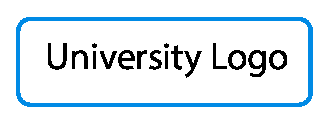
\includegraphics[height=1.5cm]{figures/logo_university}}}{}}{}%
\IfFileExists{figures/logo_institute.eps}%
{\IfFileExists{figures/logo_institute.pdf}%
  {\renewcommand{\ktx@tp@rightlogo}%
    {
\includegraphics[height=1.5cm]{figures/logo_institute}}}{}}{}%

%    \end{macrocode}
%
% Add explanation: definition
%    \begin{macrocode}
\renewcommand{\coverpagetopmargin}{1in}
\renewcommand{\coverpagebottommargin}{1in}
\renewcommand{\coverpageleftmargin}{1in}
\renewcommand{\coverpagerightmargin}{1in}
\setkomafont{titlehead}{}
\setkomafont{title}{\rmfamily\bfseries\LARGE}
\setkomafont{subject}{\rmfamily\bfseries\Large}
\setkomafont{author}{}
\setkomafont{publishers}{}
\titlehead{\ktx@tp@leftlogo\hfill\ktx@tp@rightlogo\vspace{5em}}
\subject{\ktx@tp@type}
\author{%
  prepared by\\[3mm]
  \textbf{\large \ktx@tp@author}\\[3mm]
  from \ktx@tp@address\\[5mm]
  at the \ktx@tp@institute
}
\title{\ktx@tp@title\vskip 2em\ktx@tp@titlealt\vskip 1em}

\publishers{%
\vfill
\begin{tabular}[t]{p{0.24\linewidth}p{0.76\textwidth-4\tabcolsep}}
  \bfseries Thesis number:&\begin{minipage}[t]{0.76\textwidth-4\tabcolsep}II.Physik-UniGö-MSc-2016/001\end{minipage}\\&\\
  \bfseries Thesis period:&\begin{minipage}[t]{0.76\textwidth-4\tabcolsep}1 April 2016 until 30 September 106\end{minipage}\\&\\
  \bfseries First referee:&\begin{minipage}[t]{0.76\textwidth-4\tabcolsep}\ktx@tp@firstref\end{minipage}\\&\\
  \bfseries Second referee:&\begin{minipage}[t]{0.76\textwidth-4\tabcolsep}\ktx@tp@secondref\end{minipage}\\
\end{tabular}
\vskip -3em
}
\let\@date\empty

%    \end{macrocode}
% \end{macro} 
%

% % \iffalse meta-comment
%
% ktx-toc.dtx
% Copyright 2016 Knut Zoch <knut DOT zoch AT gmail DOT com>
%
% This work may be distributed and/or modified under the conditions of
% the LaTeX Project Public License, either version 1.3 of this license
% or (at your option) any later version.  The latest version of this
% license is in http://www.latex-project.org/lppl.txt and version 1.3
% or later is part of all distributions of LaTeX version 2005/12/01 or
% later.
%
% This work has the LPPL maintenance status `maintained'.
%
% The Current Maintainer of this work is Knut Zoch.
%
% This work consists of the files kTheTex-bundle.dtx,
% kTheTex-bundle.ins, dtx/ktx-base.dtx, dtx/ktx-bibliography.dtx,
% dtx/ktx-debug.dtx, dtx/ktx-drafting.dtx, dtx/ktx-floats.dtx,
% dtx/ktx-font.dtx, dtx/ktx-headfoot.dtx, dtx/ktx-headings.dtx,
% dtx/ktx-misc-style.dtx, dtx/ktx-references.dtx, dtx/ktx-toc.dtx as
% well as the derived files ktxbbltx.sty, ktxreprt.cls and
% ktxthss.cls.
%
% \fi
%
% \iffalse
%<*driver>
\ProvidesFile{dtx/ktx-toc.dtx}
[2016/04/18 v0.1.0 ktx-toc]
%</driver>
%
%<*driver>
\documentclass[draft]{ltxdoc}
\EnableCrossrefs
\CodelineIndex
\RecordChanges
\changes{v0.1.0}{2016/04/18}{Initial version} %
\GetFileInfo{dtx/ktx-toc.dtx} %
\DoNotIndex{} %
\title{The \textsf{kTheTex-bundle} file
  \textsf{ktx-toc.dtx}\thanks{This document corresponds to
    \textsf{ktx-toc.dtx}~\fileversion, dated \filedate.}}
\author{Knut Zoch \\ \texttt{knut.zoch NOSPAM gmail.com}} %
\begin{document}
\maketitle
\DocInput{dtx/ktx-toc.dtx}
\end{document}
%</driver>
% \fi
%
% \CheckSum{0}
%
% \CharacterTable
%  {Upper-case    \A\B\C\D\E\F\G\H\I\J\K\L\M\N\O\P\Q\R\S\T\U\V\W\X\Y\Z
%   Lower-case    \a\b\c\d\e\f\g\h\i\j\k\l\m\n\o\p\q\r\s\t\u\v\w\x\y\z
%   Digits        \0\1\2\3\4\5\6\7\8\9
%   Exclamation   \!     Double quote  \"     Hash (number) \#
%   Dollar        \$     Percent       \%     Ampersand     \&
%   Acute accent  \'     Left paren    \(     Right paren   \)
%   Asterisk      \*     Plus          \+     Comma         \,
%   Minus         \-     Point         \.     Solidus       \/
%   Colon         \:     Semicolon     \;     Less than     \<
%   Equals        \=     Greater than  \>     Question mark \?
%   Commercial at \@     Left bracket  \[     Backslash     \\
%   Right bracket \]     Circumflex    \^     Underscore    \_
%   Grave accent  \`     Left brace    \{     Vertical bar  \|
%   Right brace   \}     Tilde         \~}
%
%
%
% \subsection{Table of Contents}
% \label{sec:impl-toc}
%
% The following part of the code sets up the table of contents of the
% document. This is done with the package |tocloft|.
%
% \begin{macro}{option tocloft}
%   Only load the package and change the TOC, when option
%   |tocloft=true| is given to the class. Then, change all the fonts
%   to standard serif fonts and adjust the font sizes. Remove the
%   dotted leaders completely. Change the paragraph skip (larger skip
%   above sections). Only list everything to the level of subsections
%   in the TOC (nothing below.
%
%   Currently not used is an overlapping of the sections into the
%   margin (similar to the one possible for headings). 
%    \begin{macrocode}
\ifthenelse{\boolean{ktx@tocloft}}{%
  \RequirePackage{tocloft}
  \renewcommand*{\cftchapfont}{\rmfamily\large}
  \renewcommand*{\cftsecfont}{\rmfamily\normalfont}
  \renewcommand*{\cftsecpagefont}{\rmfamily\normalfont}
  \renewcommand*{\cftsubsecfont}{\rmfamily\small}
  \renewcommand*{\cftsubsecpagefont}{\rmfamily\small}
  \renewcommand*{\cftchapleader}{\quad}
  \renewcommand*{\cftchapafterpnum}{\cftparfillskip}
  \renewcommand*{\cftsecleader}{\quad}
  \renewcommand*{\cftsecafterpnum}{\cftparfillskip}
  \renewcommand*{\cftsubsecleader}{\quad}
  \renewcommand*{\cftsubsecafterpnum}{\cftparfillskip}
  \renewcommand*{\cftpnumalign}{l}
  \setlength{\cftbeforesecskip}{1.0ex}
  \setlength{\cftparskip}{0ex}
  % \setlength{\cftsecnumwidth}{0pt}
  % \setlength{\cftsubsecindent}{0pt}
  % \renewcommand*{\cftsecpresnum}{\llap\bgroup}
  % \renewcommand*{\cftsecaftersnum}{\quad\egroup}
  \setcounter{tocdepth}{2}
}{%
  \relax
}
%    \end{macrocode}
% \end{macro} 
%

% % \iffalse meta-comment
%
% ktx-references.dtx
% Copyright 2016 Knut Zoch <github.com/knutzk>
%
% This work may be distributed and/or modified under the conditions of
% the LaTeX Project Public License, either version 1.3 of this license
% or (at your option) any later version.  The latest version of this
% license is in http://www.latex-project.org/lppl.txt and version 1.3
% or later is part of all distributions of LaTeX version 2005/12/01 or
% later.
%
% This work has the LPPL maintenance status `maintained'.
%
% The Current Maintainer of this work is Knut Zoch.
%
% This work consists of the files kTheTex-bundle.dtx,
% kTheTex-bundle.ins, dtx/ktx-base.dtx, dtx/ktx-bibliography.dtx,
% dtx/ktx-debug.dtx, dtx/ktx-drafting.dtx, dtx/ktx-floats.dtx,
% dtx/ktx-font.dtx, dtx/ktx-headfoot.dtx, dtx/ktx-headings.dtx,
% dtx/ktx-misc-style.dtx, dtx/ktx-references.dtx, dtx/ktx-toc.dtx as
% well as the derived files ktxbbltx.sty, ktxreprt.cls and
% ktxthss.cls.
%
% \fi
%
% \iffalse
%<*driver>
\ProvidesFile{dtx/ktx-references.dtx}
[2016/04/18 v0.1.0 ktx-references]
%</driver>
%
%<*driver>
\documentclass[draft]{ltxdoc}
\EnableCrossrefs
\CodelineIndex
\RecordChanges
\changes{v0.1.0}{2016/04/18}{Initial version} %
\GetFileInfo{dtx/ktx-references.dtx} %
\DoNotIndex{} %
\title{The \textsf{kTheTex-bundle} file
  \textsf{ktx-references.dtx}\thanks{This document corresponds to
    \textsf{ktx-references.dtx}~\fileversion, dated \filedate.}}
\author{Knut Zoch \\ \texttt{github.com/knutzk}} %
\begin{document}
\maketitle
\DocInput{dtx/ktx-references.dtx}
\end{document}
%</driver>
% \fi
%
% \CheckSum{0}
%
% \CharacterTable
%  {Upper-case    \A\B\C\D\E\F\G\H\I\J\K\L\M\N\O\P\Q\R\S\T\U\V\W\X\Y\Z
%   Lower-case    \a\b\c\d\e\f\g\h\i\j\k\l\m\n\o\p\q\r\s\t\u\v\w\x\y\z
%   Digits        \0\1\2\3\4\5\6\7\8\9
%   Exclamation   \!     Double quote  \"     Hash (number) \#
%   Dollar        \$     Percent       \%     Ampersand     \&
%   Acute accent  \'     Left paren    \(     Right paren   \)
%   Asterisk      \*     Plus          \+     Comma         \,
%   Minus         \-     Point         \.     Solidus       \/
%   Colon         \:     Semicolon     \;     Less than     \<
%   Equals        \=     Greater than  \>     Question mark \?
%   Commercial at \@     Left bracket  \[     Backslash     \\
%   Right bracket \]     Circumflex    \^     Underscore    \_
%   Grave accent  \`     Left brace    \{     Vertical bar  \|
%   Right brace   \}     Tilde         \~}
%
%
%
% \subsection{References}
% \label{sec:impl-refer}
%
% The following code will include the |hyperref| package, which should
% always be the last package loaded, as well as the package
% |cleveref|.
%
%
% \begin{macro}{option hyperref}
%   The package will only be loaded when the corresponding option is
%   set to |hyperref=true|. In case the user wants to add a package
%   that conflicts with hyperref if its loaded first, turn hyperref
%   off via |hyperref=false|. The following code will define some
%   colours to mark links within the document in non-standard
%   colours. Afterwards, |hyperref| is loaded with the following
%   options: 
%
% \begin{itemize}
% \item |colorlinks|: use coloured links instead of coloured boxes
%   around the links.
% \item |urlcolor|, |citecolor|, |linkcolor| set the corresponding
%   colours to the ones just defined.
% \item Link the page numbers in the TOC, instead of the chapters
%   themselves. 
% \end{itemize}
%
% If option |web| is given to the class, do everything as described
% above. For option "print", hide links, i.e. make them black again.
%
%    \begin{macrocode}
\ifthenelse{\boolean{ktx@hyperref}}{%
 \RequirePackage[%
    colorlinks = true,%
    urlcolor   = Venetian,%
    citecolor  = Lime,%
    linkcolor  = Dodger,%
    linktocpage = true,%
    ]{hyperref}
  \ifthenelse{\boolean{ktx@web}}{%
    \relax
  }{%
    \hypersetup{hidelinks}
  }  
%    \end{macrocode}
% \end{macro}
%
% \begin{macro}{cleveref}
%   Now also call the cleveref package for intelligent
%   references. They can be used via |\cref{}| commands instead of
%   |\ref{}| and include the \emph{type} of the reference within the
%   reference itself (also linked). This is achieved with the option
%   |nameinlink|. Option |capitalise| used capitalised version for
%   every type of reference, e.g. Eq. (3), Section 4, Table 3.
%
%   For some reason, some of the German reference names are not set
%   correctly, therefore some adjustments are being made.
%
%    \begin{macrocode}
  \RequirePackage[nameinlink,capitalise]{cleveref}
  \addto\captionsngerman{%
    \if@cref@abbrev
    \crefname{equation}{Gl.}{Gl.}
    \Crefname{equation}{Gleichung}{Gleichungen}
    \crefname{table}{Tab.}{Tab.}
    \Crefname{table}{Tabelle}{Tabellen}
    \fi
  }
}{%
  \relax
}
%    \end{macrocode}
% \end{macro}
%


%
%
% \PrintChanges
%
%
% \Finale
\endinput
